\section{Findings \& Discussion of Results}
\label{sec:Fin}

\subsection{Overview}
\par Section IV presents the out-of-sample results for the three portfolio strategies examined in this study: Equal-Weight, Minimum-Variance, and CVaR-minimisation at the 95\% confidence level. Results are evaluated using the seven metrics defined in Section III as the dependent variables for testing the main hypothesis, namely CAGR, annualised volatility, Sharpe ratio, Sortino ratio, VaR, CVaR, and maximum drawdown. Section IV.B reports the headline return and risk-adjusted performance of each strategy. Section IV.C then examines the downside-risk metrics directly relevant to the hypothesis. Section IV.D analyses the weight allocation patterns that underpin the observed performance outcomes. Section IV.E presents three sensitivity experiments to assess the robustness of the baseline findings. Section IV.F synthesises the results in relation to the main hypothesis, the reviewed literature, and the validity, reliability, and generalisability of the study.

\subsection{Return and Risk-Adjusted Metrics}

\begin{table*}[!t]
    \centering
    \caption{Out-of-sample performance summary.}
    \label{tab:performance-summary}
    \footnotesize
    \setlength{\tabcolsep}{5pt}
    \renewcommand{\arraystretch}{1.15}
    \begin{tabular}{l|r|r|r|r|r|r|r}
    \textbf{Strategy} & \textbf{CAGR} & \textbf{Ann.\ Volatility} & \textbf{Sharpe} & \textbf{Sortino} & \textbf{VaR 95\%} & \textbf{CVaR 95\%} & \textbf{Max Drawdown} \\ \hline
    Equal-Weight     & 5.74\% & 10.06\% & 0.555 & 0.741 & 0.95\% & 1.56\% & $-22.02\%$ \\
    Minimum-Variance & 1.61\% &  5.59\% & 0.286 & 0.392 & 0.55\% & 0.84\% & $-17.13\%$ \\
    CVaR-95          & 0.76\% &  5.46\% & 0.138 & 0.191 & 0.54\% & 0.82\% & $-20.55\%$ \\
    \end{tabular}
\end{table*}

\par Table~\ref{tab:performance-summary} summarises the out-of-sample performance of the three portfolio strategies over the 2017--2025 realised evaluation period. Although the full dataset covers 2016--2025, the first 252 trading days were used as the initial estimation window, meaning that reported portfolio outcomes begin after this first in-sample window. The table therefore reports only realised out-of-sample results.

\begin{figure}[!t]
    \centering
    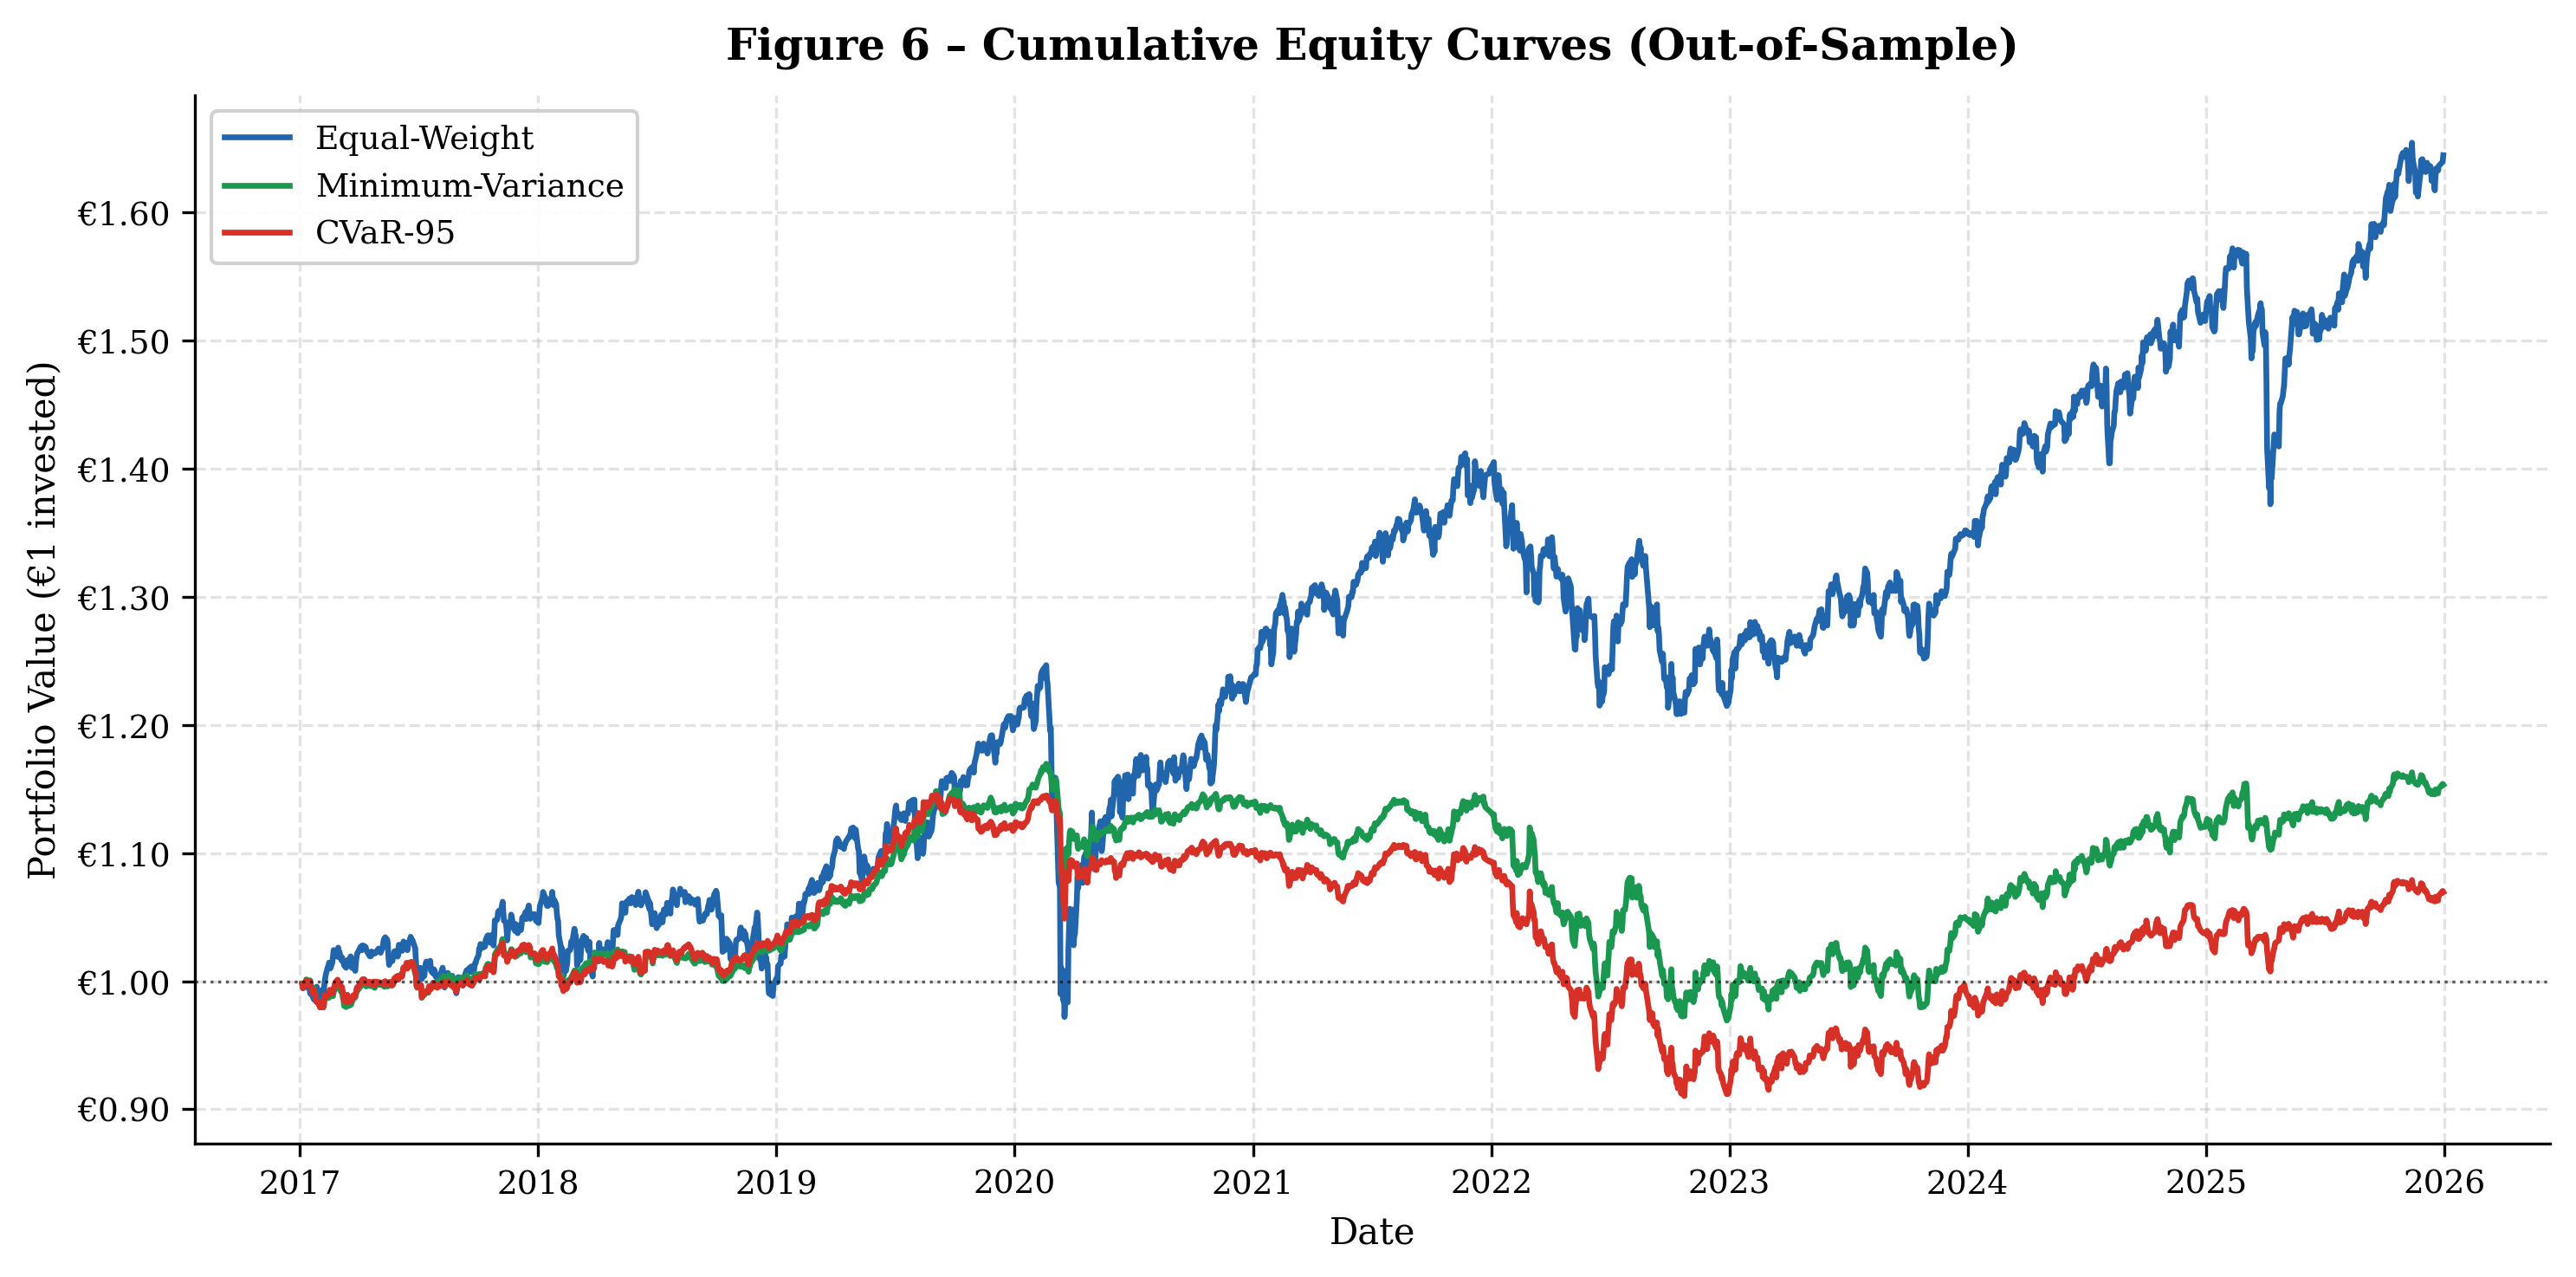
\includegraphics[width=\columnwidth]{includes/figures/06_cumulative_equity_curves.png}
    \caption{Cumulative equity curves for Equal-Weight, Minimum-Variance, and CVaR-95 portfolios over the realised out-of-sample evaluation period.}
    \label{fig:cumulative-equity-curves}
\end{figure}

\par The main return-based result is that Equal-Weight produced the strongest performance among the three strategies. It achieved the highest CAGR at 5.74\%, compared with 1.61\% for Minimum-Variance and 0.76\% for CVaR-95. It also recorded the highest Sharpe ratio of 0.555 and the highest Sortino ratio of 0.741. This indicates that Equal-Weight did not only deliver the highest return, but also the strongest conventional risk-adjusted performance in this sample. This result is also visible in Fig.~\ref{fig:cumulative-equity-curves}, where the Equal-Weight cumulative equity curve finishes above the two optimised portfolios. The supporting metrics comparison chart in Appendix A further confirms that Equal-Weight leads on the main return and risk-adjusted metrics.
\par However, this stronger return performance came with higher total volatility. Equal-Weight recorded annualised volatility of 10.06\%, almost double that of Minimum-Variance at 5.59\% and CVaR-95 at 5.46\%. This shows that the Equal-Weight portfolio accepted greater variation in returns in order to maintain broad exposure to all six ETFs. Since four of the six ETFs represented equity markets, the Equal-Weight strategy preserved a higher equity allocation throughout the out-of-sample period. This allowed it to benefit more from market upside than the two defensive strategies.
\par The lower return of Minimum-Variance and CVaR-95 is consistent with their optimisation objectives. These strategies were not designed to maximise return; they were designed to reduce variance or tail-risk exposure. Their lower volatility values show that the optimisers were successful in reducing overall return fluctuation. However, their much lower CAGR values show that this risk reduction came at a meaningful opportunity cost. In this sample, the reduction in risk did not translate into stronger risk-adjusted performance because the defensive allocation also reduced participation in equity-market growth.
\par This result is important for interpreting the hypothesis. The hypothesis did not claim that CVaR-minimisation would maximise return. Instead, it proposed that CVaR-minimisation would improve downside-risk control without material deterioration in CAGR or Sharpe ratio. The return and risk-adjusted metrics therefore already show a potential weakness in the hypothesis: CVaR-95 achieved lower volatility than Equal-Weight, but it also produced a much lower CAGR and Sharpe ratio. The next subsection therefore examines whether the downside-risk metrics are strong enough to justify this return sacrifice.

\subsection{Downside-Risk Comparison}
\par The downside-risk results provide a more direct test of the main hypothesis because the study is centred on CVaR-based risk control. In Table~\ref{tab:performance-summary}, CVaR-95 achieved the lowest VaR and CVaR values among the three strategies. Its VaR at the 95\% level was 0.54\%, slightly lower than Minimum-Variance at 0.55\% and substantially lower than Equal-Weight at 0.95\%. Its CVaR was also the lowest at 0.82\%, compared with 0.84\% for Minimum-Variance and 1.56\% for Equal-Weight. Since VaR and CVaR are reported as positive loss magnitudes, lower values indicate better short-horizon tail-risk control.
\par This finding supports one part of the hypothesis. The CVaR-minimisation objective was effective in reducing the lower tail of the daily return distribution. The improvement over Minimum-Variance was small, but it was still in the expected direction. The improvement over Equal-Weight was larger, which is consistent with the fact that Equal-Weight maintained higher equity exposure and therefore accepted greater downside variation. In this sense, the CVaR strategy behaved as expected: it reduced the short-horizon tail-loss metrics that it was designed to control.
\par However, the downside-risk result was not uniformly favourable to CVaR-95. Maximum drawdown shows a different pattern. Minimum-Variance achieved the shallowest maximum drawdown at $-17.13\%$, while CVaR-95 recorded $-20.55\%$ and Equal-Weight recorded $-22.02\%$. This means that CVaR-95 did not achieve the lowest peak-to-trough loss over the evaluation period. Fig.~\ref{fig:drawdown-comparison} also supports this distinction, as the CVaR-95 portfolio generally experienced deeper and more persistent drawdowns than the Minimum-Variance portfolio, especially from 2020 onward.

\begin{figure}[!t]
    \centering
    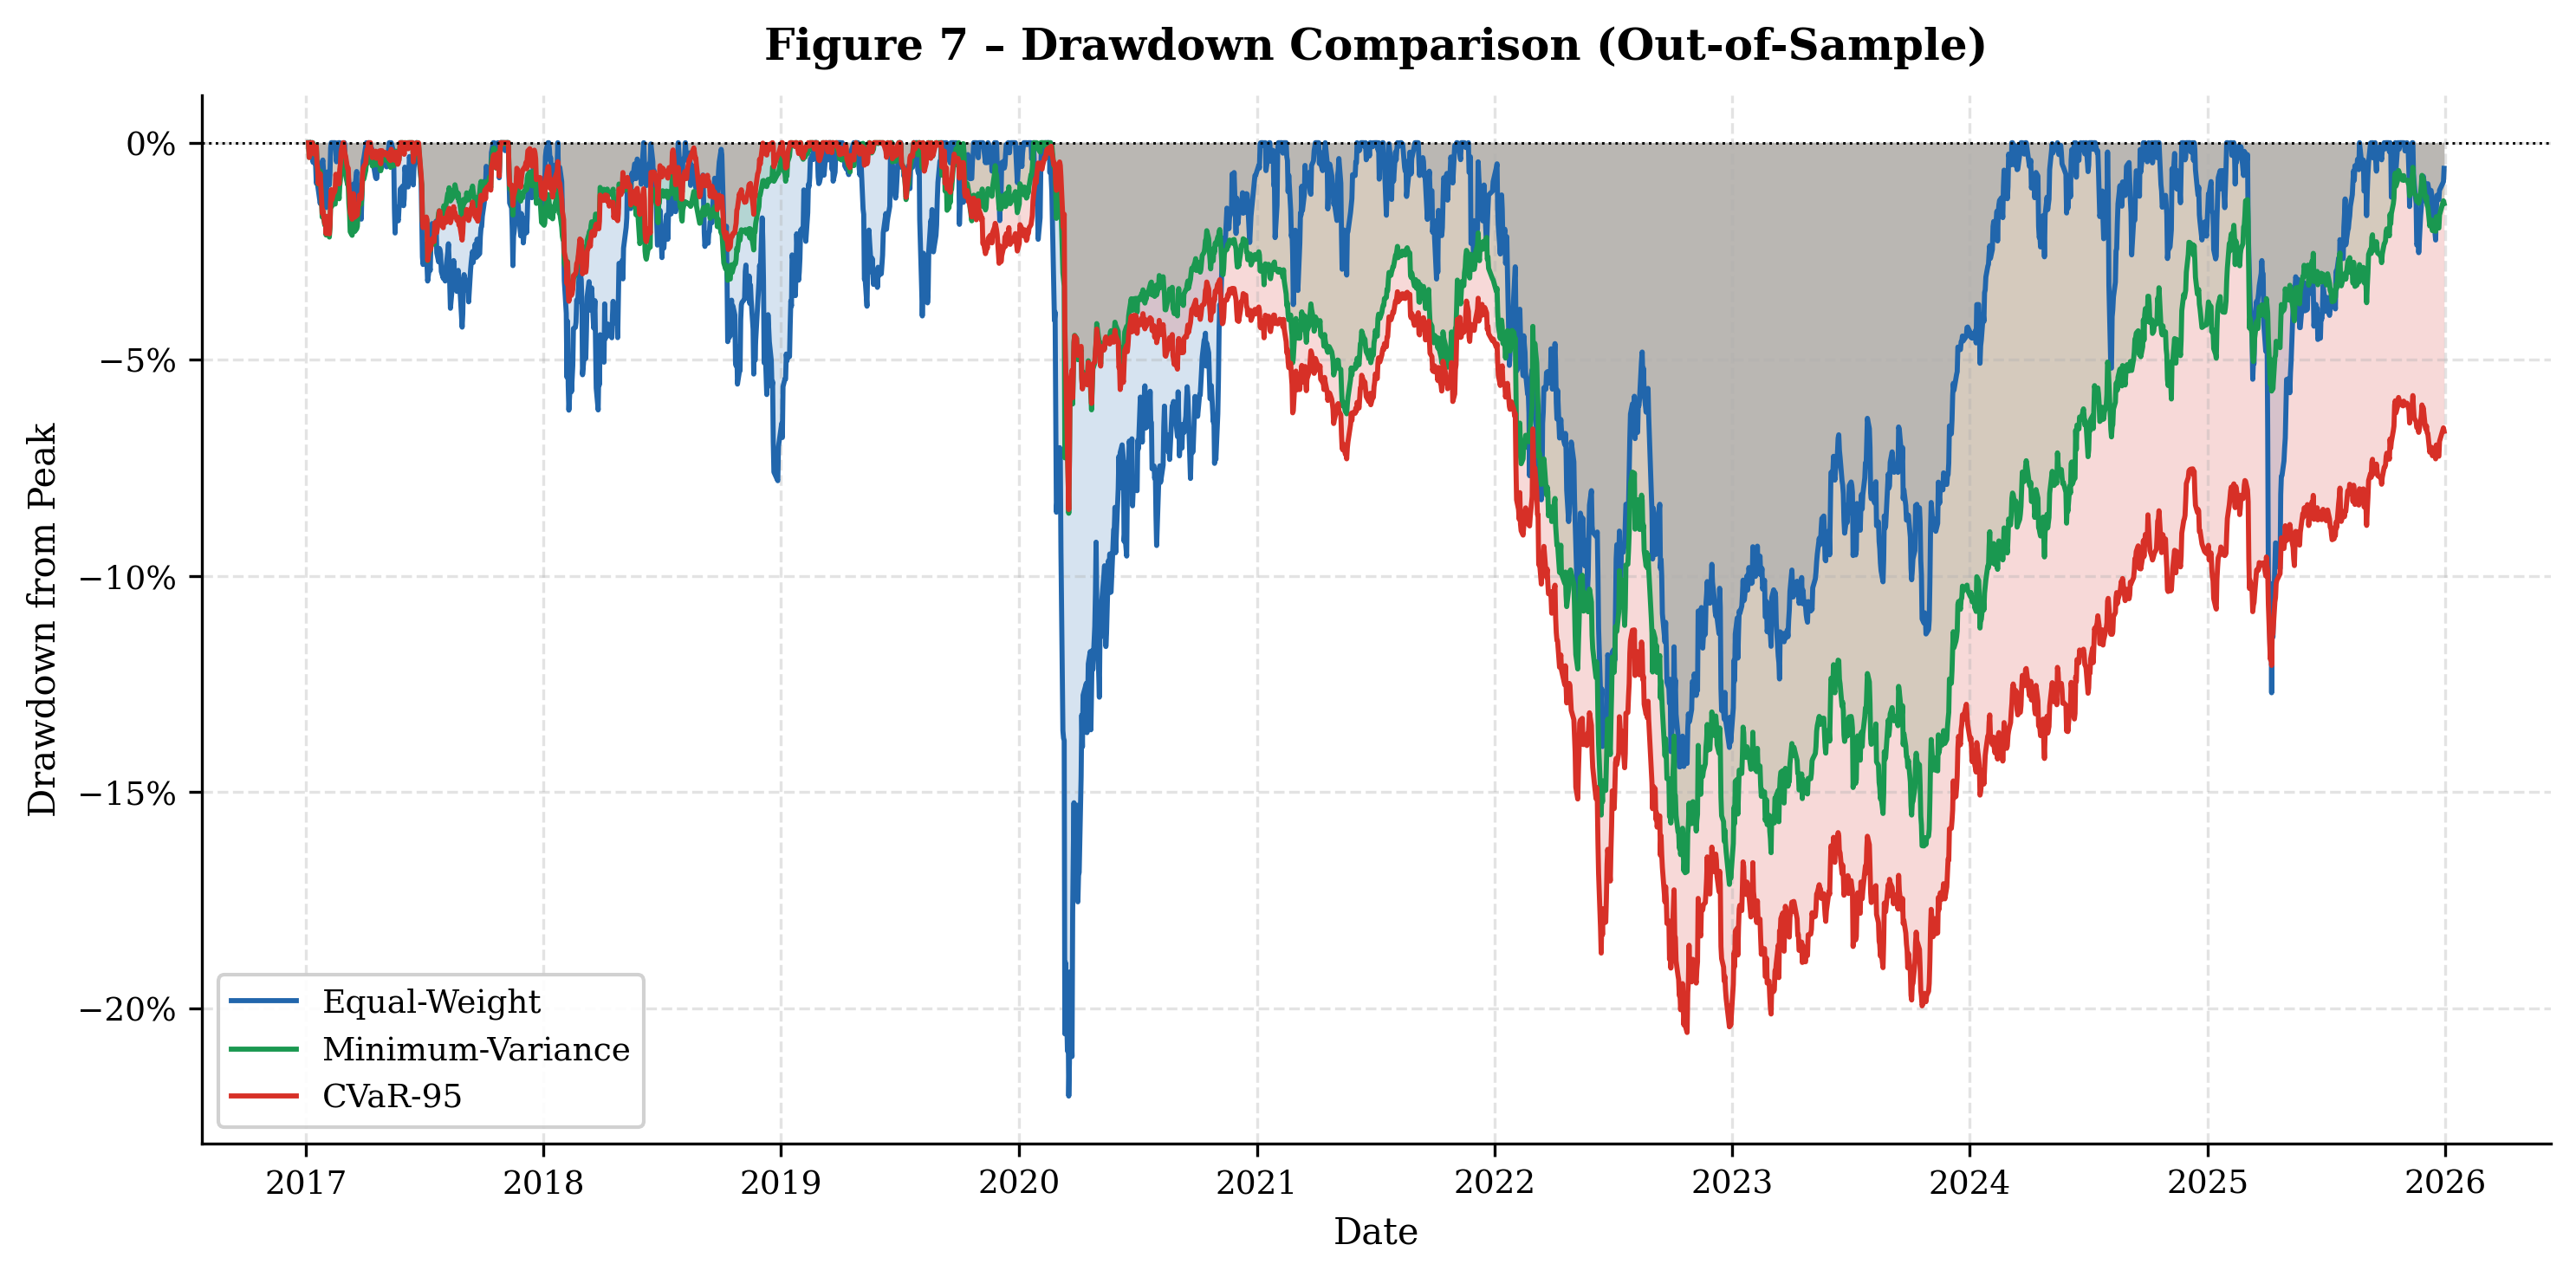
\includegraphics[width=\columnwidth]{includes/figures/07_drawdown_comparison.png}
    \caption{Drawdown comparison for Equal-Weight, Minimum-Variance, and CVaR-95 portfolios.}
    \label{fig:drawdown-comparison}
\end{figure}

\par This difference is important because VaR/CVaR and maximum drawdown measure different aspects of risk. VaR and CVaR summarise short-horizon tail losses in the return distribution. Maximum drawdown instead measures the worst cumulative decline from a previous peak. A portfolio can therefore reduce daily tail losses while still experiencing a weaker cumulative recovery path. The results show exactly this pattern: CVaR-95 performed best on VaR and CVaR, but Minimum-Variance performed best on maximum drawdown.
\par Therefore, the downside-risk evidence only partially supports the hypothesis. CVaR-95 achieved the lowest VaR and CVaR, which supports the claim that CVaR-minimisation improves short-horizon tail-risk control. However, it did not achieve the lowest maximum drawdown. As a result, the CVaR strategy cannot be described as the strongest downside-risk strategy across all risk measures. It is more accurate to state that CVaR-95 improved the specific daily tail-risk metrics it targeted, but did not dominate the Minimum-Variance benchmark on longer path-dependent downside risk.

\subsection{Weight Allocation Analysis}
\par The allocation evidence helps explain why the three strategies produced different return and risk outcomes. The detailed weight evolution plots are provided in Appendix A. Appendix A, Fig.~\ref{fig:weights-equal-weight} shows that Equal-Weight maintained a constant allocation of approximately 16.67\% to each ETF. This gave the strategy a stable combined equity exposure of around two-thirds of the portfolio, since four of the six ETFs represented equity markets. This structure explains why Equal-Weight captured more market upside and achieved the highest CAGR, but also why it carried the highest annualised volatility and higher tail-risk values.
\par By contrast, Appendix A, Figs.~\ref{fig:weights-min-variance} and~\ref{fig:weights-cvar-95} show that the optimised strategies allocated much larger weights to the two bond ETFs, especially SXRQ and, at several points, CBU0. This pattern was particularly visible in the Minimum-Variance and CVaR-95 portfolios. The allocation behaviour is consistent with the objectives of the two optimisers. Minimum-Variance reduced exposure to assets that increased portfolio variance, while CVaR-95 reduced exposure to assets that contributed more strongly to historical tail losses.
\par Appendix A, Fig.~\ref{fig:correlation-heatmap} provides further support for this behaviour through the ETF correlation heatmap. The equity ETFs were positively correlated with each other, while the bond ETFs showed lower or near-zero correlations with most equity ETFs. This made the bond ETFs useful for reducing portfolio risk. As a result, the optimised strategies shifted towards defensive assets that reduced volatility and short-horizon tail risk. This helps explain why Minimum-Variance and CVaR-95 recorded much lower annualised volatility than Equal-Weight.
\par The same allocation behaviour also explains the weaker return performance of the optimised portfolios. By concentrating more heavily in bond ETFs, Minimum-Variance and CVaR-95 reduced their exposure to equity-market growth. This was beneficial for volatility reduction, but it limited participation in the upside that drove the Equal-Weight result. The findings therefore show a clear allocation-based trade-off: the optimisers reduced risk by moving towards defensive assets, but this also reduced their ability to generate return during the out-of-sample period.
\par This allocation analysis answers the portfolio-construction research question more directly. Under identical long-only and fully invested constraints, CVaR-minimisation behaved differently from Equal-Weight and broadly similarly to Minimum-Variance. It did not create a balanced return-seeking portfolio; it created a defensive portfolio. This behaviour is consistent with a downside-risk objective, but it also explains why the strategy struggled to remain competitive on CAGR, Sharpe ratio and Sortino ratio.

\subsection{Sensitivity and Robustness}
\par Three sensitivity experiments were conducted to examine whether the baseline conclusions depended strongly on the selected backtest parameters. The tests varied the estimation window length, rebalancing frequency, and CVaR confidence level. These checks were important because the baseline specification used a 252-day estimation window, a 21-trading-day rebalance frequency, and a CVaR confidence level of 0.95. Robustness analysis therefore helped assess whether the findings were stable or mainly driven by one parameter setting.
\par The estimation-window test compared the 252-day baseline with a longer 504-day window. The longer window did not improve the main results. For CVaR-95, the Sharpe ratio declined from 0.138 under the 252-day window to 0.110 under the 504-day window. Minimum-Variance was affected more strongly, with its Sharpe ratio falling from 0.286 to 0.084. The 504-day setting also reduced the number of out-of-sample observations from 2246 to 1994, removing approximately one trading year from the realised evaluation period. This means that the longer estimation window did not provide enough benefit to justify the shorter out-of-sample period. The 252-day window was therefore retained as the more defensible baseline because it provided a full year of estimation data while preserving a longer evaluation period.
\par The rebalancing-frequency test compared the monthly baseline of 21 trading days with a quarterly alternative of 63 trading days. Equal-Weight produced identical results under both settings, with a Sharpe ratio of 0.555, a CAGR of 5.74\%, and a maximum drawdown of $-22.02\%$. This is expected because Equal-Weight uses the same constant $1/N$ target allocation and the study did not model transaction costs. CVaR-95 was also relatively stable: its Sharpe ratio changed only slightly from 0.138 to 0.130, and maximum drawdown remained close to $-20.6\%$. Minimum-Variance improved under quarterly rebalancing, with its Sharpe ratio increasing from 0.286 to 0.322 and its maximum drawdown improving from $-17.13\%$ to $-14.94\%$. This suggests that less frequent rebalancing may have reduced sensitivity to short-term covariance changes in this sample. However, the overall conclusion did not change, since Equal-Weight remained strongest on return and Sharpe performance.
\par The CVaR confidence-level test compared alpha values of 0.90, 0.95 and 0.99. CVaR-90 and CVaR-95 produced broadly similar results. CVaR-90 achieved a CAGR of 0.79\%, a Sharpe ratio of 0.147, a CVaR of 0.82\%, and a maximum drawdown of $-20.46\%$. These were close to the CVaR-95 baseline, which achieved a CAGR of 0.76\%, a Sharpe ratio of 0.138, a CVaR of 0.82\%, and a maximum drawdown of $-20.55\%$. This suggests that the baseline alpha value was not highly sensitive relative to the 90\% alternative.
\par By contrast, the 99\% confidence level was counterproductive. CVaR-99 recorded a lower CAGR of 0.23\%, a lower Sharpe ratio of 0.039, a higher annualised volatility of 5.93\%, a higher realised CVaR of 0.89\%, and a deeper maximum drawdown of $-22.56\%$. One explanation is that, with a 252-day estimation window, the 1\% tail contains only about 2.5 observations. The optimisation is therefore driven by a very small number of extreme observations in each rolling window, which can make the resulting allocation less stable out of sample. For this reason, $\alpha = 0.95$ was retained as the most defensible baseline setting.
\par Overall, the sensitivity analysis strengthens rather than weakens the baseline interpretation. CVaR-95 remained a defensive strategy under alternative window and rebalance settings, but it did not become the best return-adjusted performer. The 99\% confidence level also showed that making the CVaR objective more extreme did not improve realised tail-risk control in this dataset. The robustness evidence therefore supports the main conclusion that CVaR-minimisation reduced daily tail-risk metrics but involved a material return and Sharpe-ratio trade-off. Supporting sensitivity plots for the estimation-window, rebalancing-frequency, and CVaR-confidence-level experiments are provided in Appendix A, Figs.~\ref{fig:sensitivity-window}--\ref{fig:sensitivity-cvar-alpha}.

\subsection{Discussion}
\par The findings provide mixed evidence for the main hypothesis. The CVaR-95 strategy achieved the lowest CVaR value at 0.82\%, compared with 0.84\% for Minimum-Variance and 1.56\% for Equal-Weight. This supports the part of the hypothesis stating that CVaR-minimisation should improve tail-risk control. However, the same strategy did not achieve the lowest maximum drawdown. Minimum-Variance recorded the best maximum drawdown at $-17.1\%$, compared with $-20.6\%$ for CVaR-95. In addition, CVaR-95 suffered a material deterioration in return-adjusted performance, with a Sharpe ratio of 0.138 compared with 0.555 for Equal-Weight. The hypothesis is therefore partially supported rather than fully supported.
\par The most reasonable interpretation is that CVaR-minimisation acted as a defensive allocation rule, not as a return-maximising strategy. Its lower VaR and CVaR values show that it was effective for short-horizon tail-loss control. However, the weight evolution analysis shows that this protection was achieved by concentrating more heavily in government bond ETFs. That allocation reduced volatility and tail-risk exposure, but it also reduced participation in equity-market growth. This explains why CVaR-95 had lower annualised volatility than Equal-Weight but much lower CAGR and Sharpe performance.
\par This result is consistent with the wider portfolio-optimisation literature discussed in Section II. Mu\~{n}oz and Cifuentes \cite{munoz2026riskmetrics} show that the choice of risk metric can materially affect portfolio allocations and risk profiles, but does not necessarily guarantee simple dominance by one formulation. The present study supports that point in a smaller and more transparent UCITS ETF setting. CVaR changed the allocation and improved the specific tail-risk measure it targeted, but it did not produce superior overall performance. Similarly, Teplova et al.\ \cite{teplova2023blcopula} evaluate CVaR-based ETF portfolios using benchmark comparisons and downside-risk measures, but their framework includes additional modelling elements such as Black-Litterman views and copula-based dependence modelling. The present study shows that a simpler CVaR-minimisation design is easier to interpret, but may also be more limited in its ability to improve return-adjusted performance.
\par The findings also show why the Equal-Weight benchmark is important. Equal-Weight is simple, but it remained difficult to beat in this sample. Its constant exposure to all six ETFs allowed it to benefit from equity-market appreciation during the out-of-sample period. This does not invalidate the CVaR result, because the CVaR strategy did reduce VaR and CVaR. However, it shows that downside-risk optimisation can sacrifice too much upside when the market environment rewards equity exposure. The result therefore supports a balanced interpretation: CVaR was useful for daily tail-risk control, but Equal-Weight was superior for return and conventional risk-adjusted performance.
\par From a validity perspective, the findings are supported by the controlled experimental design. All three strategies were tested on the same ETF universe, using the same EUR-aligned return data, long-only fully invested constraints, rolling backtest logic, and evaluation metrics. This strengthens internal validity because the main intended difference between the strategies was the portfolio-construction rule. Reliability was also supported by the repeatable data preparation, backtesting, metric calculation, and sensitivity-analysis pipeline.
\par However, the findings should not be generalised beyond the scope of the study. The ETF universe contained only six UCITS ETFs, and the realised out-of-sample period was 2017--2025. Different ETF baskets, different asset classes, different fee assumptions, transaction-cost modelling, or a different market period could produce different results. The study should therefore be read as a controlled benchmark comparison in a Malta-accessible UCITS ETF context, not as universal proof that CVaR-minimisation is either superior or inferior in all portfolio settings.
\par Overall, the results answer the main research question by showing that CVaR-minimisation can improve daily tail-risk metrics compared with Equal-Weight and Minimum-Variance, but not without a material deterioration in return and Sharpe ratio. The practical implication is that CVaR-minimisation may be suitable where short-horizon tail-loss control is the main priority. However, for investors who also require competitive return and risk-adjusted performance, a simple CVaR-minimisation rule may need to be combined with additional constraints, return targets, or broader optimisation design.
